\documentclass[10pt]{beamer}
\usetheme{Warsaw}
\usepackage[T1]{fontenc}
\usepackage[utf8]{inputenc}
\usepackage{polski}
\usepackage{amsmath}
\usepackage{amsfonts}
\usepackage{amssymb}
\usepackage{amsbsy}
\usepackage{graphicx}
\usepackage{listings}
\usepackage{xcolor}
\usepackage{tikz}
\usepackage{url}
\usepackage{listings}
\usepackage{color}
\usepackage{array}

\definecolor{code}{RGB}{230,230,230}

\lstset{
    basicstyle=\ttfamily\small,
    breaklines=true,
    showstringspaces=false,
    backgroundcolor=\color{code},
    language=SQL,
    columns=fullflexible,
    keepspaces=true,
    tabsize=4,
    extendedchars=true,
    literate={ą}{{\k{a}}}1 {ć}{{\'c}}1 {ę}{{\k{e}}}1 {ł}{{\l{}}}1 {ń}{{\'n}}1 {ó}{{\'o}}1 {ś}{{\'s}}1 {ż}{{\.z}}1 {ź}{{\'z}}1
             {Ą}{{\k{A}}}1 {Ć}{{\'C}}1 {Ę}{{\k{E}}}1 {Ł}{{\L{}}}1 {Ń}{{\'N}}1 {Ó}{{\'O}}1 {Ś}{{\'S}}1 {Ż}{{\.Z}}1 {Ź}{{\'Z}}1
}

\author{Kacper Migdał, Marcin Adamski}
\title[VeloPath - Prezentacja wstępna projektu \hspace{2em}\insertframenumber/\inserttotalframenumber]{
	Prezentacja wstępna projektu aplikacji wieloplatformowej "VeloPath"
}

\logo{
\includegraphics[height=1cm]{media/logoMS.png}} 
\institute{
	
\includegraphics[height=1cm]{media/logo.jpg}\\
	Wydział Matematyki Stosowanej
}
\date{\today}  

\setcounter{tocdepth}{2}

\begin{document}
\begin{frame}
	\titlepage
\end{frame}
\section*{Agenda}
\begin{frame}
    \frametitle{Agenda}
	\tableofcontents
\end{frame} 

\section{Koncepcja projektu}

\subsection*{Główna koncepcja}

\begin{frame}
\frametitle{Główna koncepcja}
    \textbf{VeloPath} - aplikacja do wyznaczania tras rowerowych w zależności od typu roweru, umożliwiająca tworzenie pętli o wybranej długości.
\end{frame}

\subsection*{Planowane funkcjonalności}

\begin{frame}
\frametitle{Główne funkcjonalności}
    \begin{itemize}
        \item Wyznaczanie trasy w zależności od typu roweru (miejski/górski)\vspace{10pt}
        \item Tworzenie pętli o zadanej długości i wybranym miejscu startu/mety\vspace{10pt}
        \item Eksport trasy do pliku GPX\vspace{10pt}
        \item Wizualizacja trasy
    \end{itemize}
\end{frame}

\begin{frame}
\frametitle{Dodatkowe funkcjonalności}
    \begin{itemize}
        \item Możliwość wyznaczenia drogi powrotnej do startu w trakcie trasy jednym przyciskiem\vspace{10pt}
        \item Zaznaczanie odcinków drogi, które mają być unikane podczas wyznaczania tras.
    \end{itemize}
\end{frame}

\section{Porównanie z innymi systemami}

\subsection*{Istniejące systemy}
\begin{frame}
\frametitle{Istniejące systemy}
    \centering
    
\includegraphics[width=0.45\linewidth]{img/komoot_logo.png}
    \hfill
    
\includegraphics[width=0.45\linewidth]{img/strava_logo.jpg}
    \\
    
\includegraphics[width=0.3\linewidth]{img/bikemap_logo.jpg}
\end{frame}

\subsection*{Cechy różne od istniejących rozwiązań}

\begin{frame}
\frametitle{Cechy różne od istniejących rozwiązań}
    \begin{itemize}
        \item Przycisk natychmiastowego powrotu\vspace{10pt}
        \item Darmowa funkcja wyznaczania pętli o zadanej długości\vspace{10pt}
        \item Prosta budowa aplikacji
    \end{itemize}
\end{frame}

\section{Wybór technologii}

\subsection*{Technologia w budowie aplikacji}
\begin{frame}
\frametitle{Technologia w budowie aplikacji}
    \begin{table}    
        \begin{tabular}{|m{25pt}|>{\bfseries}c|m{100pt}|}
            \hline\vspace{5pt}
            
\includegraphics[width=\linewidth]{img/flutter_logo.png} & Flutter & Design aplikacji \\\hline\vspace{5pt}
            
\includegraphics[width=\linewidth]{img/flutter_map_logo.png} & Flutter Map & Wyświetlanie mapy \\\hline\vspace{5pt}
            
\includegraphics[width=\linewidth]{img/maptiler_cloud_logo.png} & MapTiler Cloud & Kafelki mapowe \\\hline\vspace{5pt}
            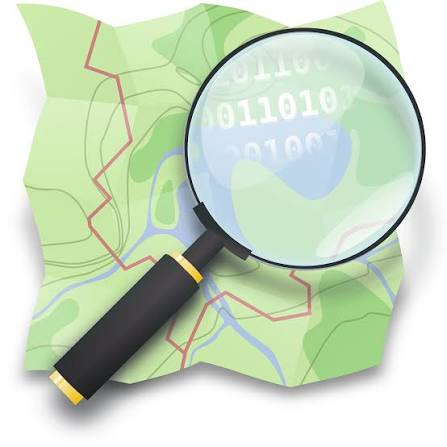
\includegraphics[width=\linewidth]{img/osm_logo.jpg} & Open Street Map & Dane drogowe \\\hline\vspace{5pt}
            
\includegraphics[width=\linewidth]{img/python_logo.png} & Python (OSMnx) & Przygotowanie grafu \\\hline
        \end{tabular}
    \end{table}
\end{frame}

\subsection*{Systemy wspomagające pracę zespołową}
\begin{frame}
\frametitle{Systemy wspomagające pracę zespołową}
    \begin{table}    
        \begin{tabular}{|m{70pt}|>{\bfseries}c|m{150pt}|}
            \hline\vspace{5pt}
            
\includegraphics[width=\linewidth]{img/github_logo.png} & Github & Zarządzanie zespołem - tworzenie zadań i harmonogramów\\\hline\vspace{5pt}
            
\includegraphics[width=\linewidth]{img/git_logo.png} & Git & Zespołowe repozytorium projektowe\\\hline
        \end{tabular}
    \end{table}
\end{frame}

\subsection*{}

\end{document}
